% Define document class
\documentclass[twocolumn]{aastex631}
\usepackage{showyourwork}

\usepackage{graphicx}
\usepackage[ruled,vlined,linesnumbered]{algorithm2e}
\usepackage{algorithmic}

\SetKwInput{Parameters}{Parameters}
\SetKwInput{Variables}{Variables}

\usepackage{tabularx,booktabs,multirow}
\usepackage{float}
\usepackage[italicdiff]{physics}

%\definecolor{rb4}{HTML}{27408B}
%\newcommand{\kw}[1]{{\color{rb4}[KW: #1 ]}}
%\newcommand{\kl}[1]{\color{cyan}[KL: #1 ]}
\newcommand{\ripple}{\texttt{ripple}}
\newcommand{\python}{\texttt{python}}
\newcommand{\jax}{\texttt{jax}}
\newcommand{\zdethp}{\texttt{zdethp}}

\newcommand{\cuhk}{\affiliation{Department of Physics, The Chinese University of Hong Kong, Shatin, N.T., Hong Kong}}
\newcommand{\flatiron}{\affiliation{Center for Computational Astrophysics, Flatiron Institute, New York, NY 10010, USA}}
\newcommand{\JHU}{\affiliation{William H. Miller III Department of Physics and Astronomy, Johns Hopkins University, Baltimore, Maryland 21218, USA}} 

% Begin!
\begin{document}

% Title
\title{Recalibrating Gravitational Wave Phenomenological Waveform Model}

% Author list
\author{Kelvin K.~H.~Lam} 
\email{kelvin33550336@gmail.com}
\cuhk
\author{Kaze W.~K.~Wong} 
\flatiron
\author{Thomas D.~P.~Edwards}
\JHU

% Abstract with filler text
\begin{abstract}
    We present a simple and general method of recalibrating gravitational wave
    (GW) phenomenological waveform models jointly. By using {\jax} and
    {\ripple}, we can perform automatic differentiation to functions, which
    allows us to use gradient-based optimization methods to recalibrate waveform
    coefficients in IMRPhenomD model. This method reduces systematic bias
    previously introduced to the model and generally can improve waveform
    accuracy. With recalibrated coefficients, we found that the typical
    \textit{mismatch} has a $50\%$ decrease. Furthermore, we analyze the
    accuracy base on the waveform's intrinsic parameters. We found that waveform
    accuracy has significant dependence on black hole spin. Reduced spin
    approximation introduces degeneracy in spin, which prevented further
    improvement. We isolated regions in the parameter space that does not fit
    the waveform ansatz. These results allow us to understand more about how to
    develop newer phenomenological models. 
\end{abstract}

% Main body with filler text
\section{Introduction} \label{sec:intro}

In the future, the Laser Interferometer Gravitational-wave Observatory (LIGO)
will finish its maintenance and start observing new gravitational wave (GW)
results. This new O4 run is expected to double the rate of current binary black
hole (BBH) observations \citep{abbott2020prospects}. Additionally, the
sensitivity of interferometers will be increased to capture more details of GW.
Having instruments with higher sensitivity, GW models of equal or higher
accuracy than observations should be used to extract GW information. Otherwise,
the extracted information would be affected more by GW models instead of
interferometer sensitivity, resulting in a bottleneck in GW analyses. Although
GW models are accurate enough for current analyses, the accuracy of current
models will no longer suffice for future data analyses
\citep{purrer2020gravitational}. Hence, it is necessary for us to develop and
improve GW models. 

% Waveform families and slight motivation of why we take Phenom model
Currently, three families of GW models are commonly used. They are the
effective-one-body (EOB) \citep{taracchini2014effective}, Numerical Relativity
(NR) surrogate \citep{varma2019surrogate} and phenomenological (Phenom) models
\citep{husa2016frequency,khan2016frequency} \kw{Add more citations related to
the newest models}. EOB models are constructed by mapping two masses onto an
effective body under an effective metric; NR surrogate models construct
waveforms using combinations of NR waveforms; Phenom models are formulated using
specific ansatz and inspiral approximations. While EOB and NR surrogate models
give better waveform approximants, Phenom waveforms can be produced much faster,
hence it is used mostly in data analysis tasks that requires many waveform
generations. This advantage scales up in data analysis tasks such as matched
filtering and parameter estimation, where many waveforms are required in each
run. This motivates us to improve upon the current framework of Phenom models,
thus can retain the advantage of fast waveform generation while improving the
model's accuracy. 

Automatic differentiation (AD) is a method to calculate derivatives of functions
up to machine precision. In traditional numerical calculations, derivatives are
usually obtained through numerical derivatives. Symbolic derivatives were
available but it was less efficient. Both methods were not viable in machine
learning, where back-propagation requires precise and rapid derivative
calculations. In {\python}, packages including \texttt{pytorch} \citep{pytorch},
\texttt{tensorflow} \citep{tensorflow2015-whitepaper}, etc. utilizes AD to train
machine learning models. AD's algorithm is intuitive in nature. Functions
defined are decomposed into tree structures of primitives, such as addition or
function evaluations. Since these operations are fundamental, they were saved as
pairs internally. Differentiation proceeds forward following the tree structure,
with the application of the chain rule in each step to evaluate its derivative.
Analytic derivatives of such operations are applied in each step and the desired
derivative can then be obtained by composing back the original function
according to the original structure. {\ripple} \citep{ripple} was a new
implementation of IMRPhenomD, one of the Phenom models. It was first implemented
in \texttt{lalsuite} using \texttt{C}. In order to make use of AD, it was
rewritten using \jax, another {\python} package that supports AD. Using
{\ripple}, one can apply AD to GW models to obtain precise derivatives, thus
allowing one to freely use derivative-based algorithms to perform data analyses. 
% Need to cite references for AD

In this paper, we investigate the possibility of further improving the accuracy
of IMRPhenomD by jointly optimizing all the fitting coefficients given NR
waveforms, and what constraints one may face when trying to further improve. We
find that simply by applying gradient descent algorithm, one can obtain a better
set of waveform coefficients, thus improving the accuracy of the model.
Furthermore, by comparing the accuracy of optimized and original waveforms, we
find that model-generated waveforms are very sensitive to their intrinsic
parameters. Specifically, IMRPhenomD favors certain parts of the parameter
space. This means IMRPhenomD introduces systematic bias to other GW analysis
tasks. This showcases the flaws of the ansatz and allows us to have a deeper
understanding of Phenom models.  
% \kw{Briefly describe the high level finding in this paper}

The rest of the paper is structured as follows: In Sec.~\ref{sec:method}, we
review the parameterization of the IMRPhenomD model and the mismatch function
that is used as an objective function for the calibration, followed by outlining the
specific optimization scheme used for recalibration. In
Sec.~\ref{sec:result}, we give the optimization result by comparing mismatches
of optimized waveforms with original waveforms. We also show how the
optimization result differs with waveforms of different intrinsic parameters. In
Sec.~\ref{sec:discussion}, we address the difference between our calibrating
procedure with \citep{khan2016frequency}. We also explain how reduced spin
parameterization affects the accuracy of the model. 

\section{Method} \label{sec:method}

\subsection{Waveform Model} \label{subsec:waveform_model}

In order to recalibrate the model, we have to understand what parameters the model has.
Here we give a succinct summary of the IMRPhenomD model and the relevant parameters.
For interested readers, please refer to \cite{khan2016frequency} for more details on construction of the model.


The IMRPhenomD model is constructed by combining three individually fitted parts
into one coherent waveform model, which consists of the inspiral, intermediate, and merger-ringdown part, 
\kw{Check if the following equation is correct. I think it is off by some smoothing factors.}
\begin{align}
	h(f,\theta)&=h_{\mathrm{ins}}(f,\theta) + h_{\mathrm{int}}(f,\theta) + h_{\mathrm{me-rd}}(f,\theta).
\end{align}

Instead of fitting the strain, which is a highly oscillatory function that is
difficult to fit, the amplitude and phase are fitted since they are smoother
functions. In each part, the amplitude and phase are made using simple functions
of frequency such as polynomials or lorentzians. These simple analytic functions
consists of parameters $\Lambda^i$, which are defined as follows. \kw{Can you
change equation one such that it consists of $\Lambda$? Also be explicit about
the form of the function used for the fitting. Like write down the polynomials
and lorentizans for the specific parts.}
\begin{align} \label{eq:Lambda}
	\Lambda^i&=\lambda_{00}^i+\lambda_{10}^i\eta \nonumber \\
	&+(\chi_{\mathrm{PN}}-1)(\lambda_{01}^i+\lambda_{11}^i\eta+\lambda_{21}^i\eta^2) \nonumber \\ 
	&+(\chi_{\mathrm{PN}}-1)^2(\lambda_{02}^i+\lambda_{12}^i\eta+\lambda_{22}^i\eta^2) \nonumber \\
	&+(\chi_{\mathrm{PN}}-1)^3(\lambda_{03}^i+\lambda_{13}^i\eta+\lambda_{23}^i\eta^2),
\end{align}
where $\lambda$ are fitting coefficients obtained during calibration, $\eta$ is
the symmetric mass ratio, and $\chi_{\mathrm{PN}}$ is the post-Newtonian spin
parameter, which is defined as 
\begin{align}
	\chi_{\mathrm{PN}}=\frac{m_1\chi_1+m_2\chi_2}{m_1+m_2}-\frac{38\eta}{113}(\chi_1+\chi_2).
\end{align}
Here, $m_{1,2}$ and $\chi_{1,2}$ are the primary and secondary mass and spin,
respectively. Finally, the individual segments are connected in a way that the
final waveform is continuous in its first derivative \kw{expand a bit}.

\kw{Need to work on this paragraph}
From Eq. \ref{eq:Lambda}, we can see that the values of $\lambda$ are
fundamental to waveform generation, which can significantly affect the shape of
final waveforms. Thus, having a set of accurate waveform coefficients is
important. Generally, waveform coefficients are obtained by calibrating with NR
waveforms, which are waveforms computed using NR simulations. In the case of
\citep{khan2016frequency}, $\lambda$ were obtained by fitting model-generated
waveforms to NR waveforms. For each NR simulation, they can obtain one set of
$\Lambda$'s through optimization. With many sets of $\Lambda$, $\lambda$ are
subsequently found by fitting against Eq. \ref{eq:Lambda}. Since the fitting
procedure is done in a piece-wise manner, the correlations between different
segments are omitted, which could limit the accuracy of the model. Also,
their calibration procedure does not guarantee to have the optimal set of
$\lambda$, since the process of connecting segments alters the previously fitted
waveform. The model-generated waveforms do not take this effect into account,
and thus introduces additional inaccuracies. 

% they did not use mismatch as the loss function

Instead, we recalibrate coefficients jointly, which we can remove inaccuracies
and biases discussed above, and can improve model accuracy. In the past, due to
the complex nature of GW strains and piece-wise formalism of IMRPhenomD,
non-linear fitting was difficult to be performed in optimizing coefficients.
Hence, piece-wise optimization was done to obtain coefficients. However, with
{\ripple} and AD from \jax, gradients of IMRPhenomD can be easily obtained, thus
allowing the use of gradient-based algorithms for us to recalibrate the model.   

\subsection{Mismatch} \label{subsec:mismatch}

To quantify the difference between waveforms, we use the standard
\textit{mismatch} $\mathcal{M}$ as the metric \citep{husa2016frequency}. It is
defined as 
\begin{align} \label{eq:mismatch}
	\mathcal{M}(h_1, h_2)=1-\max_{t_0, \phi_0}\langle \hat{h}_1, \hat{h}_2\rangle,
\end{align}
where $h_{1,2}$ represents GW strain in frequency domain, $t_0$ and $\phi_0$ are
time shift and phase shift respectively. The inner product is defined as 
\begin{align}\label{eq:inner_prod}
	\langle h_1, h_2 \rangle=4\Re\int_{f_{\mathrm{min}}}^{f_{\mathrm{max}}}\frac{h_1(f)h_2^{\ast}(f)}{S_n(f)}\,df,
\end{align}
where $\hat{h}=h/\sqrt{\langle h, h \rangle}$ is the normalized GW strain,
$S_n(f)$ is the noise spectrum, $f_{\mathrm{max}}$ and $f_{\mathrm{min}}$ are
the maximum and minimum frequencies in GW frequency spectra. 

In the original calibration \citep{khan2016frequency,husa2016frequency},
training waveforms are hybrid waveforms of NR simulations and SpinAlignedEOB
(SEOB) waveforms. The low frequency inspiral part is taken from the SEOB
waveforms while the rest of the waveforms are taken from NR simulations.
Instead, we solely use NR waveforms for comparison, since most NR waveforms used
have long enough time series data, i.e.~$>15$ orbits \citep{boyle2019sxs}, in
which they are long enough to contain part of the inspiral segment and all
merger and ringdown frequency information. We take the frequency limits as
$f_{\mathrm{min}}=0.1f_{\mathrm{RD}}$ and $f_{\mathrm{max}}=1.2f_{\mathrm{RD}}$,
where $f_{\mathrm{RD}}$ is the frequency at ringdown. This range covers most of
the IMRPhenomD's frequency range, except the minimum frequency is set higher
than that in the original calibration due to NR length. When compared with
IMRPhenomC, the frequency range is slightly extended to have a higher maximum
frequency. 

We choose to use two different noise spectra $S_n(f)$, namely the zero-detuned
high-power (\zdethp) noise spectrum and a constant spectrum. Since in any data
analysis tasks, model-generated waveforms will ultimately be used to compare
with GW observations, they are subjected to the sensitivity of detectors. Hence,
it is sensible to have waveforms calibrated with {\zdethp} spectrum rather than
a non-weighted spectrum. However, with sensitivity curve involved, we have to
choose a corresponding mass scale. Here, we simply choose $M=50M_{\odot}$ for
all waveforms, since this mass scale is common in LIGO observations. On the
other hand, we also recalibrated coefficients with the constant spectrum for a
more general purpose. 

% GW strain treatment from time-series to frequency domain
In our work, mismatches are used as a measure of discrepancies between
IMRPhenomD waveforms and NR waveforms. To compute such mismatches, NR waveforms
from the SXS catalog are taken \citep{boyle2019sxs}. These NR waveforms are
calculated using the \texttt{SpEC} code. Initially, NR waveforms are in the form
of time-series data. Since time-series data is oscillatory, performing
optimization in the time-domain is not ideal. Hence, we had chosen to transform
NR waveforms to frequency-domain to compare with IMRPhenomD waveforms with the
same intrinsic parameters. We taper the time-series using Tukey window.
\footnote{ Specifically, we choose $\alpha=2t_{\mathrm{RD}}/T$, where
$t_{\mathrm{RD}}$ is the duration of ringdown and $T$ is the duration of the
entire BBH event. } Then, the frequency spectra can be obtained by taking the
Fourier transform of the time-series. Then, mismatches can be calculated through
Eq.~\ref{eq:mismatch}~and~\ref{eq:inner_prod}. 

\subsection{Optimization Scheme} \label{subsec:optimization}

Using \ripple, we can make use of {\jax} to evaluate gradients accurately. Thus,
we can utilize simple gradient descent to recalibrate the model. 

% \kw{Mention the main advantage in this study is we can optimize everything at
% once.}

% To recalibrate the model, we have to define loss functions that quantify the
% difference between the model-generated waveforms and NR waveforms. In the
% original calibration, they took the mean square error as the loss function for
% optimization. Instead, we directly use mismatch as our metric for loss
% functions. However, the mismatch of individual waveforms is not useful in
% optimization, since it does not represent all waveforms with various intrinsic
% parameters. We ought to calibrate coefficients that suit waveforms with
% different intrinsic parameters simultaneously, hence waveforms in different
% regions of parameter space should be used in the optimization scheme. Here, we
% chose two different loss functions to examine their ability to optimize the
% model, e.g. mean of individual mismatches $\mathcal{L}_{\mathrm{mean}}$ and
% fractional loss $\mathcal{L}_{\mathrm{fl}}$. 

% Do something much more direct:
To recalibrate the model, we need to define a loss function that quantifies the
difference between the model-generated waveforms and NR waveforms. We use
mismatch over the set of all training waveforms as the loss function. While in
\citep{khan2016frequency}, they chose to use the mean square error as the loss
function, we choose mismatch as the loss function because it is closely related
to downstream objectives such as the likelihood in parameter estimation. The
mismatch is averaged over the training dataset in two ways to cover the
parameter space of interest. One of which takes a simple average and the other
takes a normalized average based on initial mismatch.

% To recalibrate the model, we need to define a loss function that quantify ...
% We use mismatch over the set of all training waveforms as the loss function.
% We choose mismatch as the loss function because it is closely related to
% downstream objectives such as the likelihood in parameter estimation. The
% mismatch is averaged over the training dataset to cover the parameter space of
% interest. (used)
\begin{align}
	\mathcal{L}_{\mathrm{mean}}&=\frac{1}{N}\sum_{i=1}^N\mathcal{M}_i \\
	\mathcal{L}_{\mathrm{fl}}&=\frac{1}{N}\sum_{i=1}^N\frac{\mathcal{M}_i}{\mathcal{M}_{i,\mathrm{ini}}},
\end{align}	
$\mathcal{M}_i$ represents the mismatch of an individual training waveform,
$\mathcal{M}_{i,\mathrm{ini}}$ represents the initial mismatch of the individual
training waveform, and $N$ is the total number of individual training waveforms.
For the first choice, it takes the mean of the mismatches, which serves as a
basic loss function. However, it is prone to be dominated by a single waveform
with a large mismatch. Other waveforms with smaller mismatches would be
insignificant comparatively, and might not be able to improve under such
optimization. Alternatively, the second choice, the mean of normalized
mismatches, eliminates the aforementioned issue. Nevertheless, it excludes the
information on initial mismatches. $\mathcal{L}_{\mathrm{fl}}$ restricts every
training waveform to decrease at similar rates, hence it is hard to obtain
optimized waveforms with mismatches in the same order of magnitude. Instead,
their ratios in mismatches would remain approximately the same. Conversely,
$\mathcal{L}_{\mathrm{mean}}$ allows the loss function to automatically adjust
and final individual mismatches would be in a similar order of magnitude. In
this paper, we display the results of using both loss functions and examine the
difference between them. 

We have chosen 11-16 NR waveforms from the set of waveforms used in the original
calibration process. Originally, 19 waveforms are taken from NR simulations for
calibrating IMRPhenomD \citep{khan2016frequency,husa2016frequency}, which they
are waveforms from the SXS catalog or BAM simulation. As BAM waveforms are not
publicly available, we cannot take the identical training set as them. Instead,
we take the available waveforms from the SXS catalog to construct our loss
function. They are listed in Tab.~\ref{tab:q148}~and~\ref{tab:q1248}. Notice the
maximum mass ratio in our training set is lower than that in
\citep{khan2016frequency}. Instead of having $q\leq18$, the maximum mass ratio
is set as 8. This is because SXS catalog does not have NR waveforms with
extremely high mass ratio. In fact, the SXS catalog only has NR waveforms with
$q\leq10$. Nevertheless, we are interested in the behavior of IMRPhenomD model
with small $q$, as most BBH events observed have $q\leq8$. Hence, we set the
maximum mass ratio to 8. 

With both mismatches, we apply gradient descent to optimize the tunable
coefficients as follows: 
\begin{algorithm}
	\caption{Gradient descent pseudocode}
	\KwIn{initial coefficients $\lambda_i$} \Parameters{number of iterations
	$N$, learning rate $\alpha$} \Variables{current coefficients $\lambda$,
	mismatch gradient $\nabla\mathcal{L}$} \KwResult{output coefficients
	$\lambda$} $\lambda\leftarrow\lambda_i$\\
	\tcc{Gradient Descent}
	\For{$i<N$}{ $\mathcal{L}\leftarrow Mismatch(\lambda)$ \\
		$\nabla\mathcal{L}\leftarrow AutoDiff(\mathcal{L})$\\
		$\lambda\leftarrow\lambda-\alpha\nabla\mathcal{L}$\\
	} \Return{$\lambda$}
\end{algorithm}
Here, $\lambda_i$ are the original coefficients given in
\citep{khan2016frequency}. We take them as the initial waveform coefficients
because they lie in the neighborhood of the minimum that we wish to find. With
such an optimization procedure, we obtain the optimized coefficients. 

\begin{figure}[t]
	\script{intrin_space.py}
	\centering
	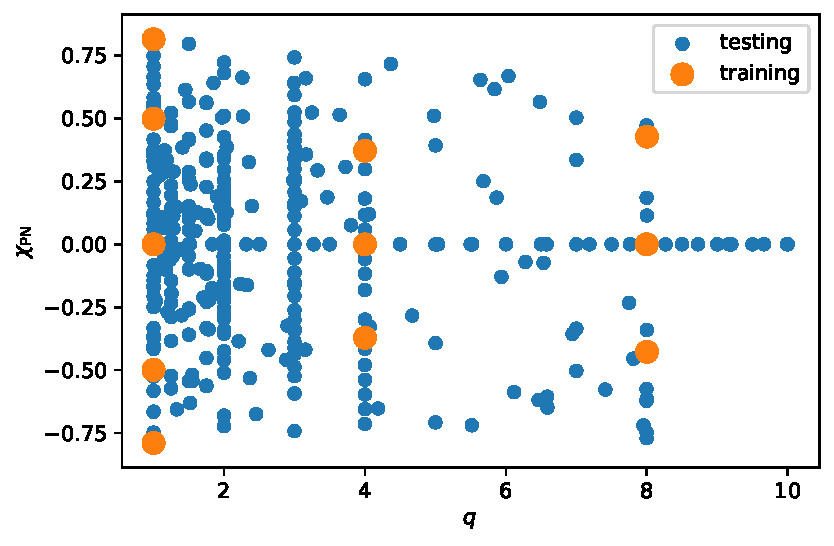
\includegraphics[width=\columnwidth]{figures/intrin_space.pdf}
	\caption{Parameter space with mass ratio against normalized reduced spin. Orange: Training waveforms; Blue: Testing waveforms}
	\label{fig:intrin_space}
\end{figure}

\begin{table}[t]
	\centering
	\begin{tabularx}{0.8\columnwidth}{@{\extracolsep{\fill}}lrrr}
		\toprule\midrule Code         & $q$ & $\chi_1$ & $\chi_2$ \\
		\midrule\midrule SXS:BBH:0156 & 1.0 & -0.95    & -0.95    \\
		SXS:BBH:0151 & 1.0 & -0.60    & -0.60    \\
		SXS:BBH:0001 & 1.0 &  0.00    &  0.00    \\
		SXS:BBH:0152 & 1.0 &  0.60    &  0.60    \\
		SXS:BBH:0172 & 1.0 &  0.98    &  0.98    \\
		SXS:BBH:1418 & 4.0 & -0.40    & -0.50    \\
		SXS:BBH:0167 & 4.0 &  0.00    &  0.00    \\
		SXS:BBH:1417 & 4.0 &  0.40    &  0.50    \\
		SXS:BBH:0064 & 8.0 & -0.50    & -0.46    \\
		SXS:BBH:0063 & 8.0 &  0.00    &  0.00    \\
		SXS:BBH:0065 & 8.0 &  0.50    &  0.46    \\ \midrule\bottomrule
	\end{tabularx}
	\caption{List of waveforms used to recalibrate the model. The mass ratio
	$q=m_1/m_2\geq 1$ with spins $\chi_{1,2}$. Out of the 11 waveforms listed
	here, 9 of them are also used in the original IMRPhenomD calibration.
	\citep{khan2016frequency} The two remaining waveforms were from BAM
	simulation, to which we do not have access.}
	\label{tab:q148}
\end{table}
\begin{table}[t]
	\centering
	\begin{tabularx}{0.8\columnwidth}{@{\extracolsep{\fill}}lrrr}
		\toprule\midrule Code         & $q$ & $\chi_1$ & $\chi_2$ \\
		\midrule\midrule SXS:BBH:0234 & 2.0 & -0.85    & -0.85    \\
		SXS:BBH:0235 & 2.0 & -0.60    & -0.60    \\
		SXS:BBH:0169 & 2.0 & 0.00     & 0.00     \\
		SXS:BBH:0256 & 2.0 & 0.60     & 0.60     \\
		SXS:BBH:0257 & 2.0 & 0.85     & 0.85     \\ \midrule\bottomrule
	\end{tabularx}
	\caption{Additional waveforms used in further recalibration.}
	\label{tab:q1248}
\end{table}

\begin{figure*}[t]
	\script{0154.py}
	\centering
	\includegraphics[width=\textwidth]{figures/0154.pdf}
	\caption{Comparison between original and optimized IMRPhenomD waveforms.
	Here shows the SXS:BBH:0154 NR waveform, which has mass ratio $q=1$ and
	$\chi_1=\chi_2=-0.8$. The original mismatch is around $2.8\times10^{-4}$ and
	the optimized mismatch is around $5.3\times10^{-5}$. Top: It shows the
	amplitude and phase of NR, original IMRPhenomD and optimized IMRPhenomD
	waveform. Bottom: It shows the relative error of amplitudes between NR and
	IMRPhenomD waveforms, and the absolute error of phases between NR and
	IMRPhenomD waveforms}
	\label{fig:0154}
\end{figure*}

\section{Result and Comparison with Original Model} \label{sec:result}

First, to judge the performance of the optimization scheme, we take $\sim530$ NR
waveforms from the SXS catalog. We choose testing waveforms with negligible
eccentricity (${e<2\times10^{-3}}$) and precession
(${\chi_{x,y}<5\times10^{-3}}$) to fit with the limitation of the model. We see
that in Fig.~\ref{fig:intrin_space}, testing waveforms have intrinsic parameters
that are within the parameter space spanned by training waveforms. Hence, we can
take these testing waveforms to compare with the original model. 

We first examine the effect of joint optimization on a single waveform. In
Fig.~\ref{fig:0154}, we can see that the optimized waveform has better accuracy
than the original waveform, especially in the inspiral region, where the
amplitude has a $50\%$ decrease in error. We have chosen one of the testing
waveforms listed in \citep{khan2016frequency} for a fair comparison. 
% In general, most waveforms within the neighborhood of the training waveforms
% show improvement in mismatches. 

Using a constant noise spectrum with $\mathcal{L}_{\mathrm{mean}}$, we compute
the mismatch for all testing waveforms and plot the distribution of the mismatch
in Fig. \ref{fig:q148}. We find the distribution's peak has shifted to the end
with a lower mismatch. Quantitatively, the peak has lowered by almost an
order-of-magnitude and the median of distribution has a $\sim50.0\%$ decrease.
Using $\mathcal{L}_{\mathrm{fl}}$, the mismatch distribution also has a similar
improvement. We see that the median of distribution has a $22.9\%$ decrease.
However, the distribution does not have a clear peak as Fig.~\ref{fig:q148}.
This is due to the problem mentioned in section \ref{subsec:optimization}.
Nevertheless, both distributions show improvement and the potential problem did
not affect the optimization scheme significantly.  

% \kw{We then compute the mismatch for all testing waveforms and plot the
% distribution of the mismatch in figure X. We find the distribution...}

\begin{figure}[t]
	\script{q148.py}
	\centering
	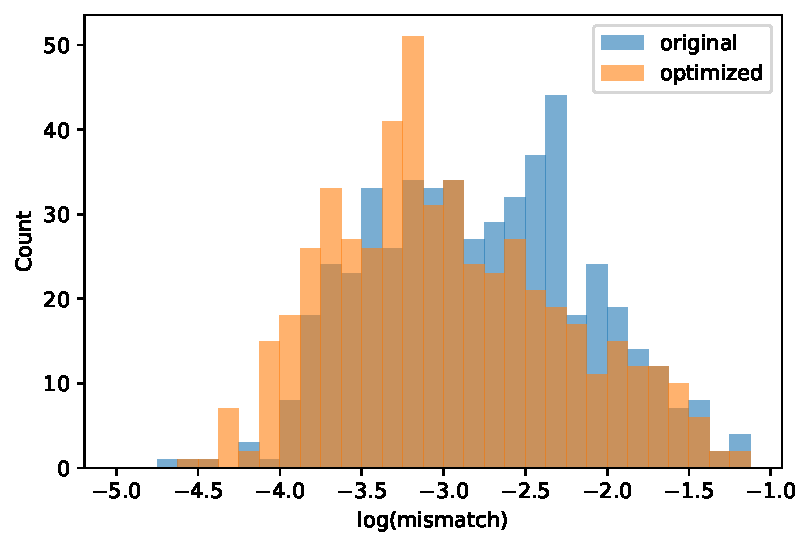
\includegraphics[width=\columnwidth]{figures/q148.pdf}
	\caption{Distributions of waveform mismatches calculated using both
	$\mathcal{L}_{\mathrm{mean}}$ and $\mathcal{L}_{\mathrm{fl}}$ in
	recalibration. We use training waveforms listed in Tab.~\ref{tab:q148} and
	mismatches are weighted with the constant noise spectrum. For the
	$\mathcal{L}_{\mathrm{mean}}$ distributions, the median decreased by 50.0\%
	while the median of $\mathcal{L}_{\mathrm{fl}}$ distribution decreased by
	22.9\%.}
	\label{fig:q148}
\end{figure}
\begin{figure}[t]
	\script{q148_q1248_compare.py}
	\centering
	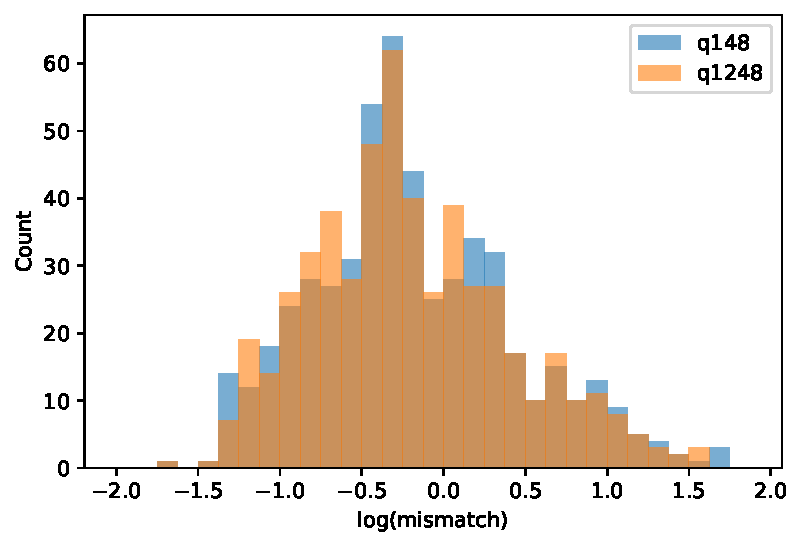
\includegraphics[width=\columnwidth]{figures/q148_q1248_compare.pdf}
	\caption{Distributions of $\log_{10}$ difference in mismatch. The
	distribution labeled \texttt{q148} uses training waveforms listed in
	Tab.~\ref{tab:q148} while the \texttt{q1248} distribution uses waveforms
	listed in Tab.~\ref{tab:q148}~and~\ref{tab:q1248}. Mismatches are calculated
	using the constant noise spectrum with the loss function
	$\mathcal{L}_{\mathrm{mean}}$.}
	\label{fig:q148_q1248_compare}
\end{figure}

Similarly, using the same procedures, distributions of mismatches calculated
using {\zdethp} noise spectrum show better improvement than the weighted
mismatch. The shape of the distribution is similar to Fig.~\ref{fig:q148}. This
effect is expected since the IMRPhenomD model was originally constructed and
fitted using the {\zdethp} weighted mismatch. Thus, it should be a model that
fits closely to the NR waveforms with the influence of {\zdethp} noise spectrum
instead of the constant spectrum. 

With the success of improving waveforms, we increase the number of training
waveforms for optimization. Taking additional waveforms listed in
Tab.~\ref{tab:q1248}, we obtain a new set of coefficients. We see in Fig.
\ref{fig:q148_q1248_compare}, new waveforms produced only have a very small
improvement. The high mismatch tail of the optimized distribution remains
similar in length and endpoint as the original distribution, meaning that they
cannot be improved using our procedure. Likewise, using additional waveforms to
optimize loss function with {\zdethp} spectrum shows the same result, where the
new distribution barely shows any improvement. 

% We believe that either the ansatz does not suit waveforms within certain
% regions of parameter space or the set of optimized coefficients falls to a
% minimum where they do not fit some testing waveforms. If in some region of
% parameter space, the ansatz does not fit well with NR waveforms, it would
% never be able to have consistent improvement under optimization. Instead, it
% would surf around the loss manifold with random fluctuations in mismatches. If
% the set of coefficients does not fit, then dividing the parameter space into
% regions and fitting separate sets of coefficients should give better results.

Given the ansatz used in the waveform model is unlikely to be fully compatible
with NR, and the optimization procedure is done over a distribution of waveforms
with different source parameters, it is conceivable that there are some
trade-off in accuracy of the waveform models between different part of the
parameter space. If this is the reason why the high mismatch tail is not
improving during the joint-optimization, separating the parameter space into
smaller subspace should help alleviate this issue. On the other hand, if the
ansatz does not have the right parameterized form to capture the behavior of the
NR waveforms as a function of the intrinsic parameters, the result should be
always biased, and we should not expect any improvement even if we separate the
parameter space into smaller space during training.

Since we know intrinsic parameters play an important role in the ansatz, we
would like to investigate how intrinsic parameters affect the recalibration
process. First, we plot the parameter space of $q$ vs. $\chi_{\mathrm{PN}}$ in
Fig. \ref{fig:ps_q148_qchi}. In the low mass ratio region, waveforms with both
positive and negative log differences are mixed up. On the other hand, along the
horizontal line $\chi_{\mathrm{PN}}=0$, waveform mismatches consistently improve
under recalibration. 

Furthermore, we plot the parameter space of $\chi_1$ vs. $\chi_2$ in
Fig.~\ref{fig:ps_q148}. Waveforms along the diagonal axis, i.e.
$\chi_1\approx\chi_2$, show good mismatch improvements. We expect to see this
feature since the original coefficients were fitted using NR waveforms with
equal or similar spin, hence the model prefers waveforms with similar spin. One
interesting feature is how the second and fourth quadrants respond to
optimization. In the second quadrant ($\chi_1<0$ and $\chi_2>0$), waveforms
generally improve with along optimization. However, mismatches in the fourth
quadrant ($\chi_1>0$ and $\chi_2<0$) do not improve after optimization. Most
waveforms even turned worse after optimization. These waveforms correspond to
the waveforms in the high mismatch tail in Fig.~\ref{fig:q148}. 

% Waveform mismatches in the fourth quadrant, i.e. $\chi_1>0$ and $\chi_2<0$,
% performed worse after optimized. IMRPhenomD is constructed using single spin
% parameter, where there are degeneracy between $\chi_1$ and $\chi_2$. In
% regions with opposite extreme spin components, degeneracy significantly alters
% intrinsic parameters passed into waveform generation, hence the fourth
% quadrant shows such feature. 

\begin{figure}[t]
	\script{ps_q148_qchi.py}
	\centering
	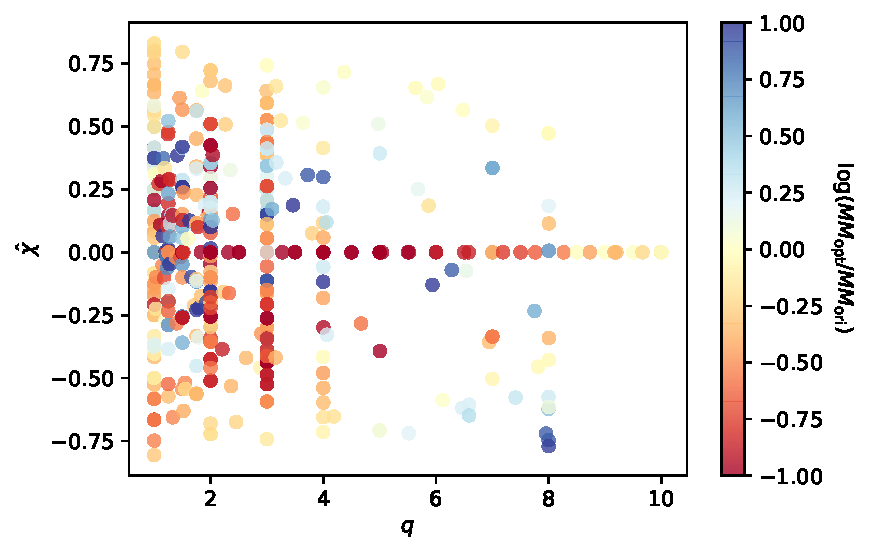
\includegraphics[width=\columnwidth]{figures/ps_q148_qchi.pdf}
	\caption{Parameter space of testing waveforms of
	$q$~vs.~$\chi_{\mathrm{PN}}$. We use the recalibrated result from
	$\mathcal{L}_{\mathrm{mean}}$ with the constant noise spectrum and training
	waveforms in Tab.~\ref{tab:q148}. Here, the colorbar represents the
	$\log_{10}$ difference between optimized and original unweighted
	mismatches.}
	\label{fig:ps_q148_qchi}
\end{figure}
\begin{figure}[t]
	\script{ps_q148_chi1chi2.py}
	\centering
	\includegraphics[width=\columnwidth]{figures/ps_q148_chi1chi2.pdf}
	\caption{Parameter space of testing waveforms of $\chi_1$~vs.~$\chi_2$. We
	use the recalibrated result from $\mathcal{L}_{\mathrm{mean}}$ with the
	constant noise spectrum and training waveforms in Tab.~\ref{tab:q148}.}
	\label{fig:ps_q148}
\end{figure}

\begin{table}[t]
	\centering
	\begin{tabularx}{0.8\columnwidth}{@{\extracolsep{\fill}}lrrr}
		\toprule\midrule Code         & $q$ & $\chi_1$ & $\chi_2$ \\
		\midrule\midrule SXS:BBH:0172 & 1.0 & 0.98     & 0.98     \\
		SXS:BBH:0152 & 1.0 & 0.60     & 0.60     \\
		SXS:BBH:0001 & 1.0 & 0.00     & 0.00     \\
		SXS:BBH:1417 & 4.0 & 0.40     & 0.50     \\
		SXS:BBH:0167 & 4.0 & 0.00     & 0.00     \\
		SXS:BBH:1426 & 8.0 & 0.48     & 0.75     \\
		SXS:BBH:0167 & 8.0 & 0.00     & 0.00     \\ \midrule SXS:BBH:0370 & 1.0
		& -0.20    & 0.40     \\
		SXS:BBH:2092 & 1.0 & -0.50    & 0.50     \\
		SXS:BBH:0330 & 1.0 & -0.80    & 0.80     \\
		SXS:BBH:2116 & 2.0 & -0.30    & 0.30     \\
		SXS:BBH:2111 & 2.0 & -0.60    & 0.60     \\
		SXS:BBH:0335 & 2.0 & -0.80    & 0.80     \\
		SXS:BBH:0263 & 3.0 & -0.60    & 0.60     \\
		SXS:BBH:2133 & 3.0 & -0.73    & 0.85     \\
		SXS:BBH:0263 & 4.0 & -0.80    & 0.80     \\ \midrule SXS:BBH:0156 & 1.0
		& -0.95    & -0.95    \\
		SXS:BBH:0151 & 1.0 & -0.60    & -0.60    \\
		SXS:BBH:0001 & 1.0 & 0.00     & 0.00     \\
		SXS:BBH:1418 & 4.0 & -0.40    & -0.50    \\
		SXS:BBH:0167 & 4.0 & 0.00     & 0.00     \\
		SXS:BBH:1419 & 8.0 & -0.80    & -0.80    \\
		SXS:BBH:0063 & 8.0 &  0.00    &  0.00    \\ \midrule SXS:BBH:0304 & 1.0
		& 0.50     & -0.50    \\
		SXS:BBH:0327 & 1.0 & 0.80     & -0.80    \\
		SXS:BBH:2123 & 2.0 & 0.30     & -0.30    \\
		SXS:BBH:2128 & 2.0 & 0.60     & -0.60    \\
		SXS:BBH:2132 & 2.0 & 0.87     & -0.85    \\
		SXS:BBH:2153 & 3.0 & 0.30     & -0.30    \\
		SXS:BBH:0045 & 3.0 & 0.50     & -0.50    \\
		SXS:BBH:0292 & 3.0 & 0.73     & -0.85    \\ \midrule\bottomrule
	\end{tabularx}
	\caption{List of waveforms used in recalibrating coefficients in 4 quadrants. From top to down are the first, second, third and fourth quadrants. Note that for the first and third quadrants, waveforms are chosen to have equal or similar spins, while the training waveforms for the second and fourth quadrants are chosen to have opposite spins.}
	\label{tab:quadrants}
\end{table}

As we see in Fig.~\ref{fig:ps_q148} that the recalibration procedure is
significantly different in different regions in the parameter space, we split
the parameter space into 4 quadrants and perform separate fitting with training
waveforms listed in Table \ref{tab:quadrants}. Note that in the second and
fourth quadrants, there are not enough waveforms with $q>4$, hence the result
are only valid up to $q\leq4$. From Fig.~\ref{fig:ps_q148_quadrant}, we see that
all waveforms, except those in the fourth quadrant, show improvement in
mismatch. Many features seen in Fig.~\ref{fig:ps_q148} can be found here again.
First, we focus on waveforms with the same spin direction, i.e.
$\chi_1\chi_2>0$. Waveforms lying in the neighborhood of the diagonal axis have
noticeable improvements in mismatch due to most training waveforms being
equal-spin waveforms. For the second quadrant, waveforms improved significantly
with only a few defects due to some testing waveforms having $q>4$. In the
fourth quadrant, most optimized waveforms have a higher mismatch than the
original waveforms, as indicated by the positive log difference of mismatches.
As performing optimization in a smaller subspace does not show any improvement
compared to the original result, the ansatz mostly does not fit waveforms in the
fourth quadrant. 

\begin{figure}[t]
	\script{all_quadrants.py}
	\centering
	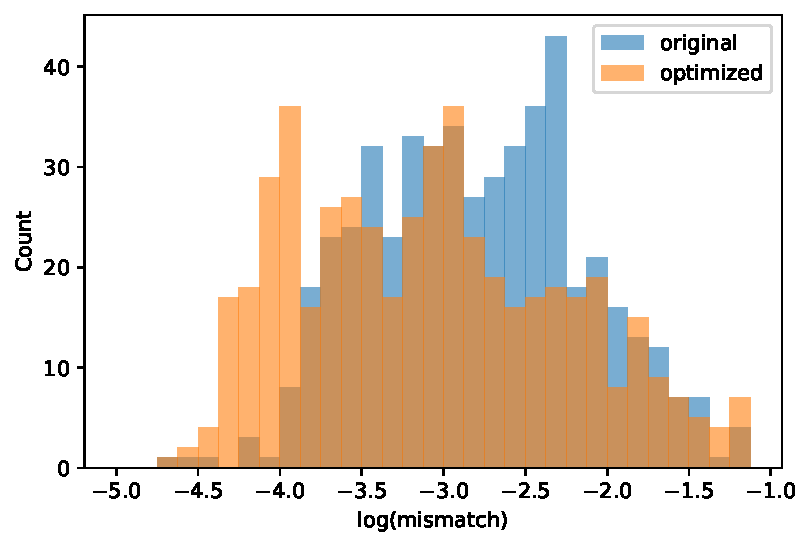
\includegraphics[width=\columnwidth]{figures/all_quadrants.pdf}
	\caption{Distributions of mismatches after optimizing in separate quadrants.
	We use a constant noise spectrum to calculate mismatch and
	$\mathcal{L}_{\mathrm{mean}}$ for the loss function. Generally, most
	waveforms with mismatch $>10^{-2}$ lies in the fourth quadrant. }
	\label{fig:all_quadrants}
\end{figure}

\begin{figure}[t]
	\script{ps_q148_quadrants.py}
	\centering
	\includegraphics[width=\columnwidth]{figures/ps_q148_quadrants.pdf}
	\caption{Parameter space of testing waveforms. Each quadrant is fitted independently. Colorbar represents log difference of mismatches before and after optimization.}
	\label{fig:ps_q148_quadrant}
\end{figure}

\section{Discussion} \label{sec:discussion}

%\begin{enumerate} \item Comparison with the original paper is not the same.
%   (Different waveforms, different ways to modify the waveform, different range
%   of frequencies) \item More waveforms are taken so it should be more robust,
%   since the parameter space coverage is better. \item Problems with IMRPhenomD
%   model, i.e. $\chi_{\mathrm{eff}}$ reduces the dimension of spin space
%   $\chi_1, \chi_2$, so the model is flawed. Comparison issues. (Caveat) \item
%   Can in principle split parameter space into regions that can be separately
%   optimized. If not, then its must be the model's problem. Would the region
%   classification be made automatic. Are there any algorithms to do so? \item
%   Future work (Repeat on other GW models. Mapping between NR surrogate to see
%   any systematics.) \end{enumerate}

We have shown the result of recalibrating waveform coefficients. One thing to
note is that our recalibration procedure is not exactly the same as the original
calibration. For instance, we use a different set of NR waveforms, frequency
range, etc. Nonetheless, as the decrease in mismatch is rather significant, this
optimization procedure should be able to improve the accuracy of IMRPhenomD on a
similar scale regardless of the differences. Here, this result serves as a
demonstration of the general method used.  
% In Fig.~\ref{fig:0154}, the error in the inspiral region is around halved for
% both amplitude and phase. Similarly, for the merger-ringdown region, the
% optimized waveforms also show great improvement. 

We see that in Fig.~\ref{fig:q148_q1248_compare}, performing optimization with
more training waveforms only has a small increase in the accuracy of the
waveform model. We believe that by increasing the number of waveforms, the
accuracy will not have a significant change as the waveform coefficients are
already over-determined. Using more calibration NR waveforms will not further
improve the model significantly. This suggests the form of the parameterized
ansatz is not suitable for certain regions in the parameter space, thus
mismatches of only a few waveforms decreased while other waveforms remain at the
high mismatch tail with little changes. This implies that the model is
ultimately restricted by the flexibility of the ansatz. 

One of the major problems causing inaccuracy in the ansatz is the reduced spin
approximation. In IMRPhenomD, it is modeled using a single spin parameter,
namely $\chi_{\mathrm{PN}}$ as outlined in Sec. \ref{sec:method}. Parameterizing
a BBH merger with one spin parameter introduces degeneracy within the parameter
space. Events with distinct black hole spins could result in equal
$\chi_{\mathrm{PN}}$, thus generating the same waveform. Especially with high
unequal spin events, $\chi_{\mathrm{PN}}$ would identify them as the same as
events with small spin, thus giving an inaccurate result. Generally, the
approximation gives straight lines of degeneracy in the parameter space, with
its slope (always negative) dependent on the mass ratio. From
Fig.~\ref{fig:ps_q148}, we see that along a degeneracy line, the ansatz behaves
better in the top left region than the bottom right. To try to accommodate this
issue, we split the parameter space into 4 quadrants as described in Sec.
\ref{sec:result}. However, even with separate optimizations, we see in
Fig.~\ref{fig:ps_q148_quadrant} that the fourth quadrant still shows similar
mismatches as before while the second quadrant further improved. This suggests
the ansatz is region-specific, with a higher preference for BBH events with
$\chi_1<0$ and $\chi_2>0$. 

Separating regions into 4 quadrants is done purely out of simplicity. To give a
more comprehensive analysis, one should be systematic about region selection.
One can use level set estimation algorithms to obtain systematic regions of
interest. This general algorithm reveals further degeneracies or issues within
the ansatz. Then, recalibrating such individual regions might give better
results. Alternatively, one can select regions according to the lines of
degeneracy. However, with limited NR waveforms, such a selection scheme is not
viable for us. In the future, with more NR waveforms spanning the entire
parameter space, one can perform optimization with fewer restrictions. 

While our work focused mainly on the IMRPhenomD model, this simple yet general
method can be utilized in other differentiable GW models. For instance, within
the same family, IMRPhenomX \citep{pratten2020setting} or IMRPhenomP
\citep{hannam2014simple} models. By jointly fitting a new set of coefficients,
it is expected that both models can be improved since they are constructed in a
similar way as the IMRPhenomD model. For example, they also use PN approximant
as part of the ansatz in the inspiral segment. One interesting result might
arise while recalibrating IMRPhenomX model \citep{pratten2020setting}. Since it
is parameterized by an additional anti-symmetric spin parameter, it is expected
to not show the same degeneracy as described above. Further analysis might give
insights into the systematics of Phenom models. Moreover, this method can be
applied to other GW model families, such as NR surrogate models
\citep{varma2019surrogate} or EOB models \citep{taracchini2014effective}. NR
waveform calibration procedures could be made easier and are likely to improve
current models.

% Can we further check systematic bias by injection? But how can we know the
% real mass or spin in the first place if we disregard GW models.

\section{Conclusion} \label{sec:conclusion}

In this paper, we have presented a systematic method to recalibrate GW models.
This method utilizes {\jax}'s automatic differentiation to apply
derivative-based optimization to recalibrate GW models jointly. Using the new
implementation of the IMRPhenomD model, {\ripple}, which is written in \jax, in
conjunction with NR waveforms from the SXS catalog, we recalibrate waveform
coefficients of the IMRPhenomD model. In general, the waveform accuracy can be
improved by 50\%. Comparing {\zdethp} weighted and unweighted mismatch, weighted
mismatches have a slightly better improvement. In contrast, different types of
loss function result in significantly different final mismatch distributions,
where the result can be seen in Fig.~\ref{fig:q148}. By increasing the number of
training waveforms, we see a slight improvement increase in
Fig.~\ref{fig:q148_q1248_compare}. 

Furthermore, we investigated how the intrinsic parameters affect the
improvement. Fig.~\ref{fig:ps_q148} shows that the optimization procedure has a
certain preference for waveforms lying in the second quadrant while the fourth
quadrant cannot be improved. To further test this result, we recalibrate
waveforms in separate regions in parameter space. As shown in
Fig.~\ref{fig:ps_q148_quadrant}, this recalibration process gives further
improvement to the second quadrant while the fourth quadrant shows similar
result. This indicates that the model's ansatz does not fit waveforms in the
fourth quadrant. This phenomenon is due to the reduced spin approximation used
in parameterizing the ansatz, where degeneracies between $\chi_1$ and $\chi_2$
are introduced. 

While we naively separate the optimization process into 4 quadrants, one can
perform systematic region-selection. In principle, we can apply this general
method to other newer and more accurate models such as IMRPhenomX or IMRPhenomP
models. Then, we can perform all the above analyses to understand how to
construct better GW Phenom models in the future.  

% From analyzing mismatches in parameter space, we investigated the accuracy of
% generated waveforms based on their mass ratio and spin. Similar studies can be
% performed on other GW models to give better criteria to 

% Improved the IMRPhenomD model. Found regions that can be improved. Checked
% ansatz. 

\section{ACKNOWLEDGMENTS}


\bibliography{bib}

\end{document}
